\section{仿真实验与分析}
本章介绍了在Ubuntu系统下本文使用的强化学习路径规划和深度强化学习车道保持算法实验结果,具体内容如下所示。
\subsection{路径规划仿真}
\subsubsection{仿真环境}
路径规划仿真所用环境为Python+gym,gym为Python强化学习库。具体为使用Ubuntu20.04系统,在Pycharm中利用Python建立了一个gym风格的环境来进行强化学习
路径规划。此环境可以理解为供强化学习进行迭代训练的“地图”,在这个环境中智能体每做出一个动作,环境都会给出在当前状态下的奖励。
对于强化学习而言此环境是必须的,在本文的程序中,奖励函数在环境中给出。
\subsubsection{Qlearning路径规划}
Qlearning路径规划效果图
如图~\ref{fig:4-1}。
\begin{figure}[H]
  \centering
  \includegraphics[width=0.8\linewidth]{fig/qlearning.png}
  \caption{\textbf{Q-leaning路径规划}}
  \label{fig:4-1}
\end{figure}
可以看到基于Qlearning算法可以成功规划出路径,此路径对比最短路径差距不大,且可以通过定制
奖励函数的方式,实现基于 用户的个性化路径规划。因为本文所用的奖励函数的原则为距离的远近,
所以可以看出路线中较多的使用了直线,拐弯集中发生于障碍物附近。由此可以看出采用Q学习的算法
,路径规划的结果可以达到设计之初的要求,这与强化学习的机制有关。
\begin{figure}[H]
  \centering
  \includegraphics[width=0.5\linewidth]{fig/q_path_length.pdf}
  \caption{\textbf{Q-leaning奖赏路径长度图}}
  \label{fig:4-2}
\end{figure}
路径规划过程中奖赏趋势图,与路径长短随时间变化图
如图~\ref{fig:4-2},可以看到随着迭代轮数的增加,在500epochs左右路径长度和奖励收敛,
之后出现的尖峰是因为是因为执行$\epsilon$贪心策略产生的。因为本文设计
的奖励函数与路径长度相关,所以从图中可以看到其收敛的一致性于对称性。
\subsubsection{SARSA路径规划}
SARSA路径规划效果图
如图~\ref{fig:4-3},可以看到SARSA算法规划出的路径和Q学习规划出的路径长短相差不大。
\begin{figure}[H]
  \centering
  \includegraphics[width=0.8\linewidth]{fig/sarsa1.png}
  \caption{\textbf{SARSA路径规划}}
  \label{fig:4-3}
\end{figure}
路径规划过程中奖赏趋势图,与路径长短随时间变化图如图~\ref{fig:4-4},从图中可以看出,SARSA算法在1000epochs左右收敛,但之后尖峰出现较多,
且幅值较大。对比来看,
Q学习的收敛速度大于SARSA,迭代过程的波动也小于SARSA,所以综合来看,Q学习更实用于路径规划。
\begin{figure}[H]
  \centering
  \includegraphics[width=0.8\linewidth]{fig/sarsa_path_length.pdf}
  \caption{\textbf{SARSA奖赏路径长度图}}
  \label{fig:4-4}
\end{figure}

\subsection{DQN车道保持}
\subsubsection{数据预处理}
本文DQN车道保持主要使用了Carla中的语义相机,数据预处理也是主要对语义相机的数据进行处理。首先使用将Carla中的语义标签进行缩减,缩减细节详见本文第二章CARLA中的传感器。
得到缩减后的含有标签数据的Carla语义相机数据后,并使用PIL和Pytorch对图像数据进行尺寸统一化处理,并将其转化成张量送到神经网络中。这样做的目的主要是为了加快模型的训练速度,
并抑制过拟合现象。此外,本文还将Carla中的车辆控制简化为一些离散的控制指令,作为神经网络的输出,即DQN的动作空间。具体为向左向右转向22度,直行。
\subsubsection{车道保持实验结果}
DQN车道保持奖赏图
如图~\ref{fig:4-5}。可以看出随着迭代轮数的增加,奖励值在一定范围内波动最终收敛于0,收敛于0即沿着车道行驶,中间极值的出现是因为车辆运行$\epsilon$贪心策略导致撞到障碍物所以给出了较大的负值奖励,从图中可以看出本文已基本实现了车道保持任务。
\begin{figure}[H]
  \centering
  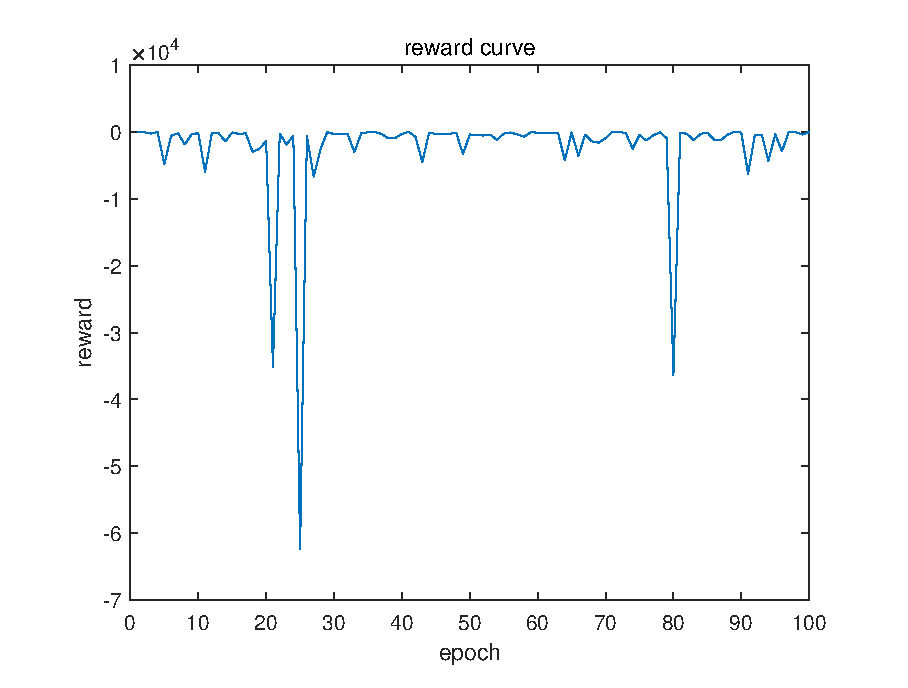
\includegraphics[width=0.5\linewidth]{fig/reward.eps}
  \caption{\textbf{DQN车道保持奖赏图}}
  \label{fig:4-5}
\end{figure}

\subsection{本章小结}
本章主要介绍了强化学习路径规划与深度强化学习车道保持的实验结果,对结果进行了分析。可以看到强化学习路径规划可以很好的体现出奖励函数的要求,基本可以实现本文提出的
“以人为本”的路径规划。针对深度强化学习车道保持,在Carla仿真环境下进行了测试,其结果表明将深度强化学习引入无人驾驶决策模块具有一定可行性。